\chapter{The FET programme in Horizon 2020}
This chapter describes the FET initiative as part of the Horizon 2020 scheme. Lorem ipsum dolor sit amet, consectetur adipisci elit, sed eiusmod tempor incidunt ut labore et dolore magna aliqua. Ut enim ad minim veniam, quis nostrum exercitationem ullam corporis suscipit laboriosam, nisi ut aliquid ex ea commodi consequatur. Quis aute iure reprehenderit in voluptate velit esse cillum dolore eu fugiat nulla pariatur. Excepteur sint obcaecat cupiditat non proident, sunt in culpa qui officia deserunt mollit anim id est laborum.

\section{The Horizon 2020 funding programme}
Horizon 2020 is the biggest Research and Innovation funding programme financed by the European Union to date. It aims at ensuring a smart and sustainable societal and economic growth by investing on and applying scientific research. The programme has a total budget of nearly 80 billions euro over a seven-year period (from 2014 to 2020).

Horizon 2020 is Europe's eighth Research and Innovation programme in chronological order. Previous programmes were each four years long, with the first started in 1984. The increasing budget allocated for the Research and Innovation programmes is shown in figure \ref{FP_funds}.

\begin{figure}[!t] 
 \begin{center}
 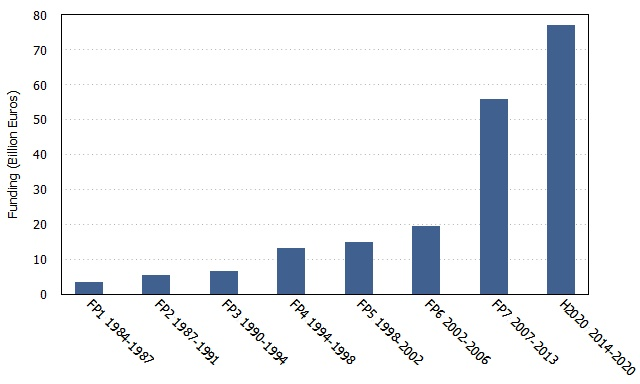
\includegraphics[scale=0.4]{Images/FP_funds.jpg}
 \caption{Budget allocated for Europe's Research and Innovation programmes in billion euros over the past years. FP stands for Framework Programme. Data from \cite{OECD}.}
 \label{FP_funds}
 \end{center}
\end{figure}

%data from https://ec.europa.eu/research/fp7/pdf/fp-1984-2013_en.pdf#view=fit&pagemode=none

Any natural or legal persons such as universities, research organisation, companies etc. can apply for funding from Horizon 2020. Applications must fit into one of the following categories: 

\begin{itemize}
 \item \textbf{Excellent science:} the goal of this initiative is to support and increase the excellence of European scientific research on a global level in a variety of fields.
 \item \textbf{Industrial leadership:} this class of projects targets the development of the technological innovations of tomorrow's market and the growth of European small and medium enterprises.
 \item \textbf{Societal challenges:} this group focuses on priorities of the European society such as health, education, energy supply and food by combining knowledge and methods from different scientific fields and humanities.  
 \item \textbf{European Institute for Innovation and Technology (EIT):} the EIT is an independent European body supporting European growth by promoting synergies among three key societal players: education, research and business. 
 \item \textbf{Euratom:} this pillar focuses on nuclear research and safety with to the goal to contribute to the decarbonisation of the energy supply.
\end{itemize}

The budget breakdown of the Horizon 2020 into the aforementioned lines of action is shown in figure \ref{H2020_budget_breakdown}

\begin{figure}[!t] 
 \begin{center}
 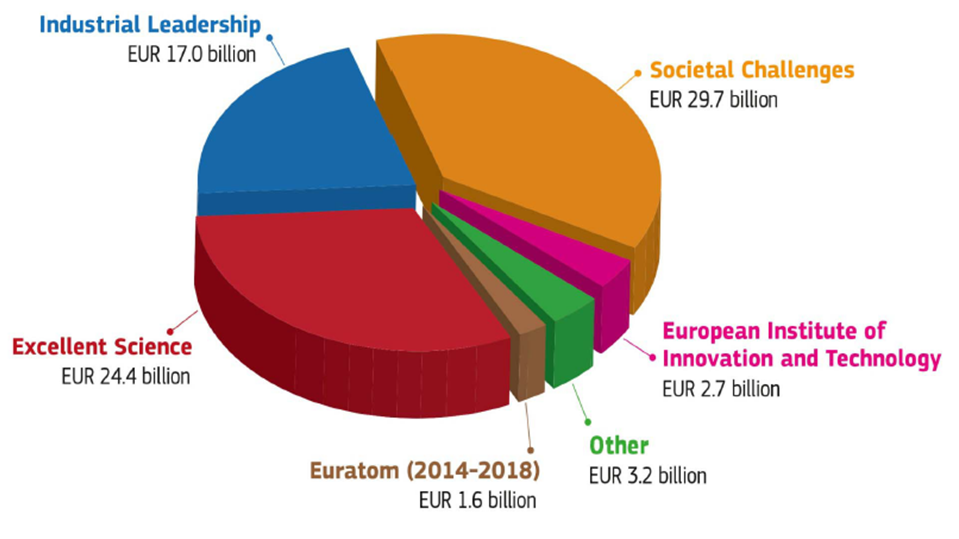
\includegraphics[scale=0.3]{Images/H2020_budget_breakdown.png}
 \caption{Budget breakdown of the Horizon 2020 programme. Original image in \cite{OECD}.}
 \label{H2020_budget_breakdown}
 \end{center}
\end{figure}


%\begin{table}[h!]
%\begin{center}
%  \begin{tabular}{ccc}
%     \hline 
%     \hline
%     \ \ & \ S5-VSR1 \ & \ S6-VSR2/3 \\ 
%     \hline
%     \hline
%     Networks \ & \ H1H2L1V1 and H1H2L1 \ & \ H1L1V1 and H1L1 \\
%     Observation time (days) \ & \ 60.0 + 238.9 = 298.9 \ & \ 42.1 + 79.7 = 121.8 \\
%     Best search range (Mpc) \ & \ 241 (H1H2L1V1) \ & \ 228 (H1L1V1) \\
%     Total-mass range $(\text{M}_{\odot})$ \ & \ $[100, \, 450]$ \ & \ $[50, \, 450]$ \\ 
%     Mass-ratio range \ & \ $[1:4, \, 1:1]$ (EOBNRv2) \ & \ $[1:6, \, 1:1]$ (EOBNRv2) \\ 
%      \ & \ \ & \ $[1:10, \, 1:1]$ (IMRPhenomB) \\ 
%     Spin range $(\chi)$ \ & \ - \ & \ $[- 0.8, \, 0.8]$ \\ 
%     \hline
%     \hline
%  \end{tabular}
%\end{center}
%\caption{Comparison of the S5-VSR1 and S6-VSR2/3 searches. The table focuses on the considered networks, the accumulated observation time, the largest search ranges achieved and on the investigated IMBHB parameter space.}
%\label{S5_S6_comparison}
%\end{table}